\section{Computational Results}\label{sec:compResults}

In this section, we aim at studying mainly the cost and the computing time of the CHARP for the overall 32 data instances of the ROADEF 2009 Challenge. To obtain the computing time, we run all 32 instances simultaneously and we retrieve the computing time of the last one being solved. As for the cost we use the cost checker application provided by the ROADEF 2009 Challenge. To better understand the latter we will also compute the total amount of delay, cancelled flights, new flights and, taxi flights. The remainder of this section consists of, Section \ref{sec:impact} where we will demonstrate the impact of adding new flights and taxi flights. Since the heuristic performs a pincer movement in Section \ref{sec:pincerSpeed} we will determine which is the best speed by changing the decremental and incremental steps.\\
 
%All the models and algorithms were written in Python language. The scripts were implemented on a computer with 4-core processors running at 2.3  GHz and 16 GB memory.\\


\subsection{The Impact of New Flights and Taxi Flights}\label{sec:impact}
To study the impact of new flights we define the base scenario in table \ref{tbl:baseScenario}. 

	\begin{table}[h!]
		\centering
		\caption{Base Scenario}
		\label{tbl:baseScenario}
		\begin{tabular}{ll}
			\hline
			Domain step {[}min{]} & 60                           \\
			Upper bound           & $3.0 \times 10^{12}$ \\
			Upper bound step      & $1.0 \times 10^{11}$ \\
			Lower bound           & $4.0 \times 10^4$ \\
			Lower bound step      & $1.0 \times 10^4$ \\
			\hline
		\end{tabular}
	\end{table}

In  figure \ref{fig:flightNoFlight}, we can observe that the aggregate cost is lower for the heuristic that has new flights and taxi flights added, than for the one with none of them added. This result was expected since adding new flights or taxi flights consists of adding new arcs which in turn can increase the flow of the flight network. It is possible to observe a similar result for the maximum time to obtain a solution. The latter can be explained on a series of cascading effects: adding new flights will decrease the available airport capacity, which in turn will decrease the size of the domains hence resulting in the decrease of the size of search space to be traversed. We  observe that extending the time window results increases the total amount of delay of the solution. As for the total number of cancellations we verify that it is lower for the heuristic that has new flights and taxi flights added, than for the one with none of them added. This observation is in line with the aggregate cost. Finally we point out that the total number of new flights is in the order of magnitude of 125 and the total number of taxi flights is in the order of magnitude of 200. Both values do not change substantially with the size of the time window.

	\begin{figure}[h!]
		\centering
		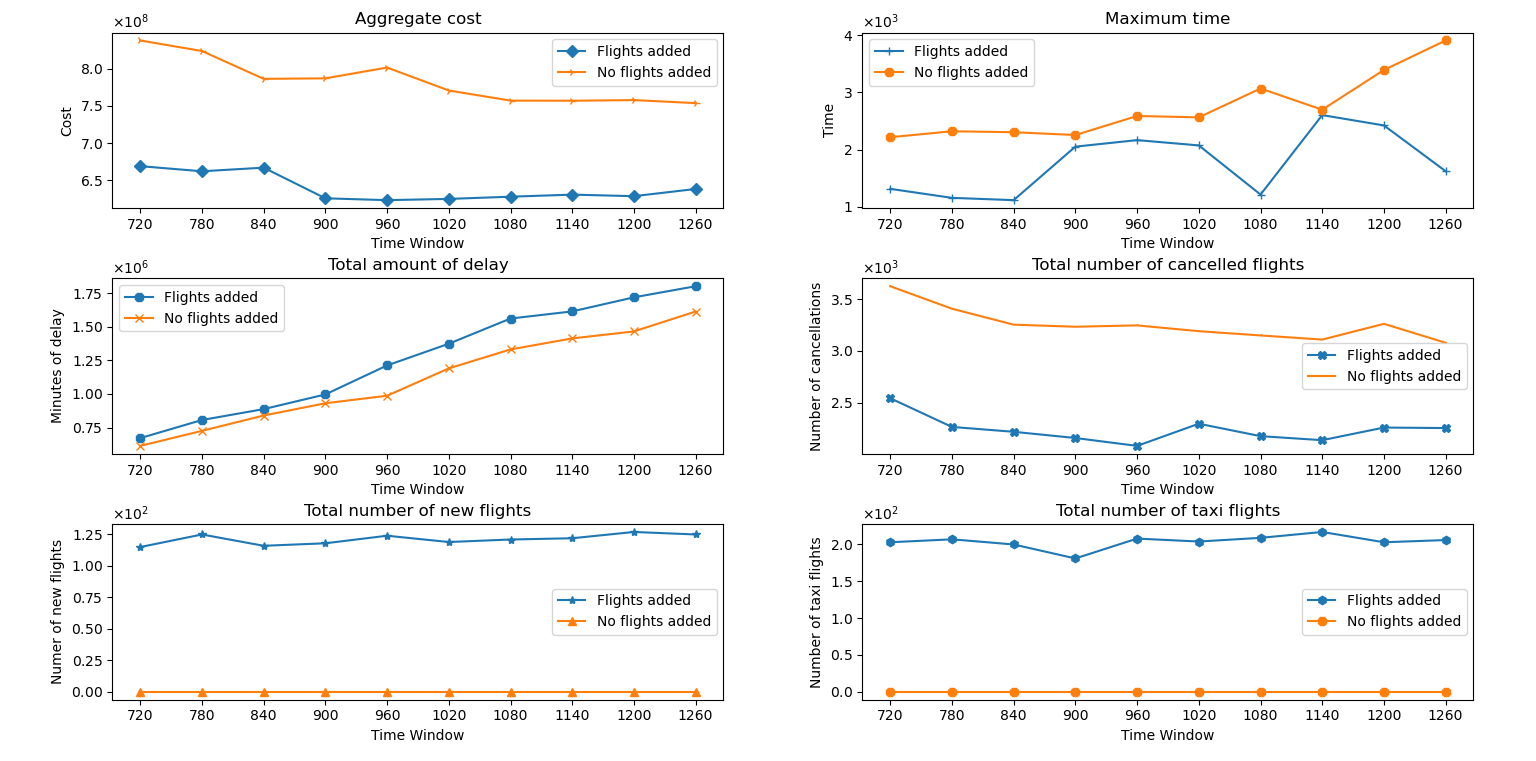
\includegraphics[width=\textwidth]{figures/flightNoFlight2x3.png}
		\caption[]{The Impact of New Flights and Taxi Flights}
		\label{fig:flightNoFlight}
	\end{figure}


\subsection{The Impact of the Pincer Speed}\label{sec:pincerSpeed}
To study the impact of the pincer speed we define the set of incremental and decremental steps in table \ref{tbl:pincerSpeed}.

	\begin{table}[h!]
		\centering
		\caption{Base Scenario}
		\label{tbl:pincerSpeed}
		\begin{tabular}{lll}
			\hline
			& Incremental step size     & Decremental step size      \\
			Speed 0.5 & $0.5 \times 10^{4}$ & $0.5 \times 10^{11}$ \\
			Speed 1   & $1.0 \times 10^{4}$ & $1.0 \times 10^{11}$ \\
			Speed 2   & $2.0 \times 10^{4}$ & $2.0 \times 10^{11}$ \\
			Speed 3   & $3.0 \times 10^{4}$ & $3.0 \times 10^{11}$ \\
			Speed 4   & $4.0 \times 10^{4}$ & $4.0 \times 10^{11}$ \\
			Speed 5   & $5.0 \times 10^{4}$ & $5.0 \times 10^{11}$ \\
			\hline
		\end{tabular}
	\end{table} 

In figure \ref{fig:speed} we can observe that the minimum aggregate cost is obtained for speed 1 in the 960 minutes times window.	
	\begin{figure}[h!]
		\centering
		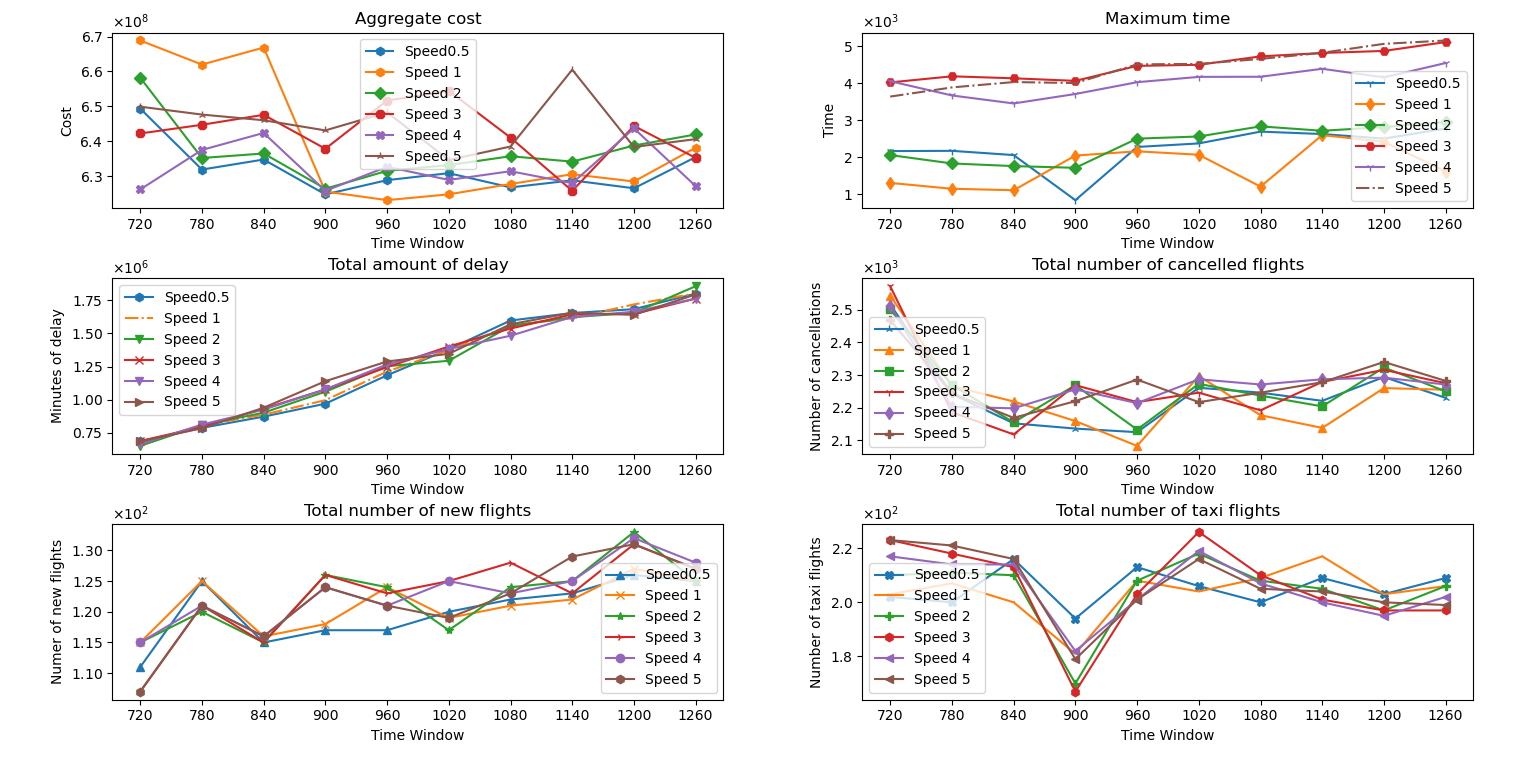
\includegraphics[width=\textwidth]{figures/speed2x3.png}
		\caption[]{The Impact of the Pincer Speed}
		\label{fig:speed}
	\end{figure}

	\begin{figure}[h!]
		\centering
		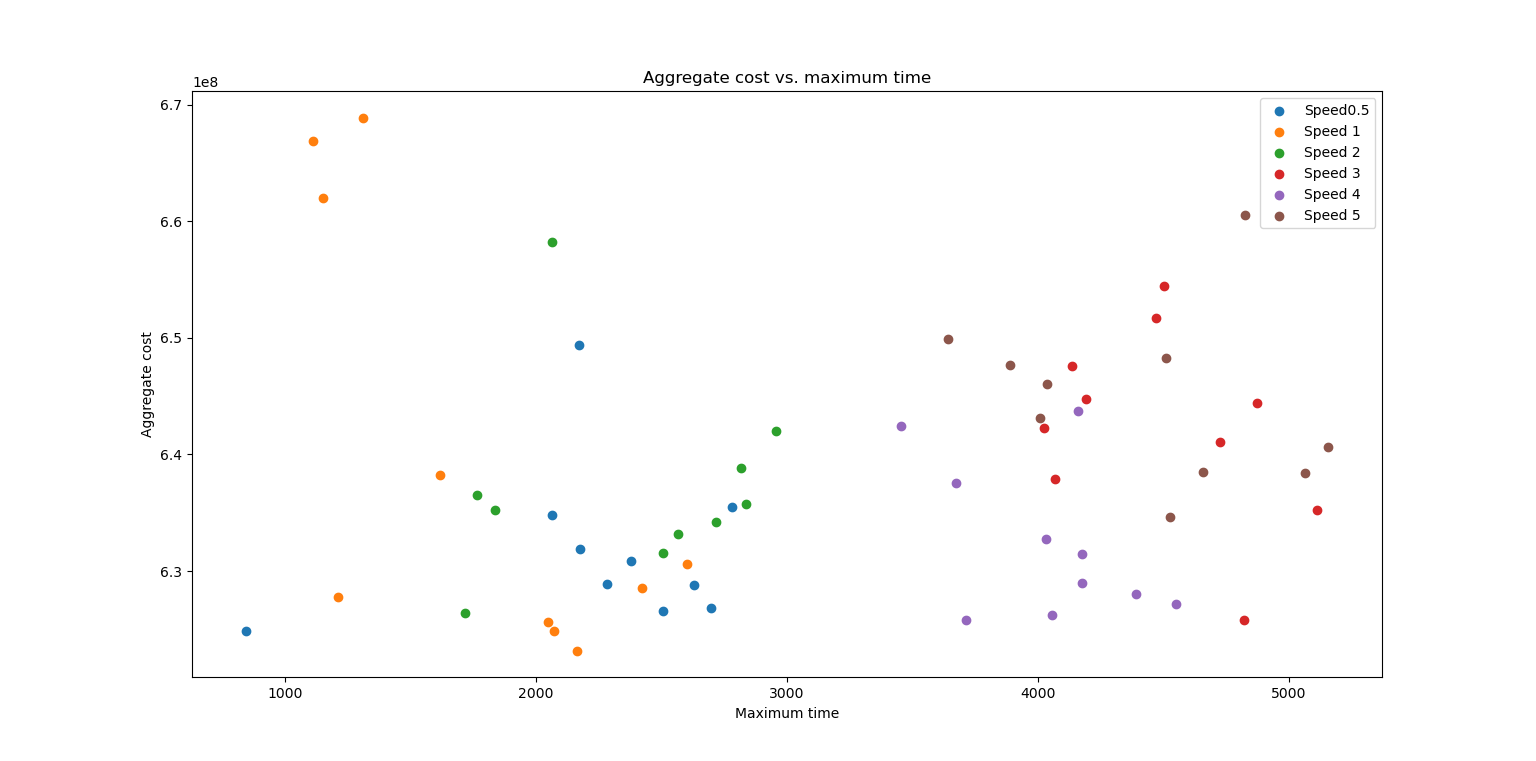
\includegraphics[width=\textwidth]{figures/costTime.png}
		\caption[]{The Paretto Front}
		\label{fig:costTime}
	\end{figure}


